\chapter{Averaging procedure}




\section{Buchert's approach}

This is a bare-bones approach to the averaging problem, doing a direct averaging of scalar measurable quantities, under a spatial hypersurface. The first papers of Buchert started by assuming a "dust" like spacetime\cite{Buchert_2000}\cite{Buchert_2001}, he recently adapted this approach with an extensive generalised spacetime\cite{Buchert_2020} and foliation, which is fully described in Figure \ref{fig:foliation}.
   
In a synchronous frame, the inhomogeneous and anisotropic metric is $ds^2=-dt^2+h_{ij}dx^idx^j$. The average of any scalar quantity over a spatial hypersurface of constant proper time, $\Sigma$, is,
\begin{equation}
	\langle S(t,x)\rangle_{\Sigma}\equiv \frac{1}{V_{\Sigma}(t)}\int_{\Sigma} d^3x \sqrt{h}S(t,x),
    \label{eqn:cbuchert_average}
\end{equation}

The commutative relation between the time derivative and the averaging operator is given by,
\begin{equation}
	[\partial_t \cdot, \langle\cdot \rangle_{\Sigma}] S=\langle \Theta S\rangle_{\Sigma}-\langle \Theta\rangle_{\Sigma}\langle S\rangle_{\Sigma},
	\label{eqn:comoving_commutation_rule_buchert}
\end{equation}
where $\Theta$ is the expansion rate of the dust, assuming the dust is comoving with the observer. The scale factor is defined as $a_{\Sigma}\propto V_{\Sigma}^{1/3}$, and so $\langle\Theta\rangle_{\Sigma}=3\partial_t \ln a_{\Sigma}$.



\begin{figure}[h]
	\centering
	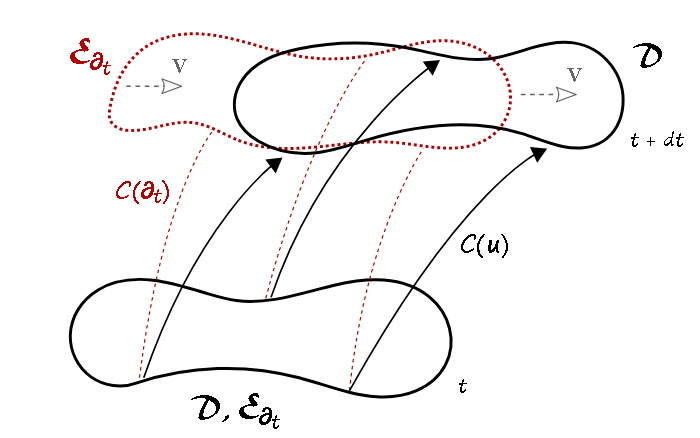
\includegraphics[scale=0.5]{domain_transportation.png}
\end{figure}

\textcolor{blue}{Aqui seguimos buchert, mas aplicamos para a congruencia de $n^\mu$}

This figure represents how the hypersurface $\Sigma$ is transported along the congruence $C(n)$, with $X^i=\text{const.}$. 
And is transported along the congruence $C(\partial_t)$, with $x^i=\text{const.}$, which coincides with $\Sigma$ at the time $t$. 
The domain undergoes a spatial motion, with velocity $\mathbf{\beta}$, in the coordinate basis $(t,x^i)$. Therefore $d/dt$ and $\int_\Sigma d^3x$ do not commute.

Consider a family of maps, $\bm{\Phi}_t=\mathbf{f}(t,\cdot)$, in order to change the coordinates $x^i$ to $X^i$,
\begin{equation}
	x^i = f^i(t,\mathbf{X}), \qquad d^3x = \text{det}\left(\frac{\partial \mathbf{f}(t,\mathbf{X})}{\partial \mathbf{X}}\right)d^3X = J(t,\mathbf{X})d^3X,
\end{equation}
while the domain transforms as, $\Sigma_x \rightarrow \Sigma_X = \mathbf{\Phi}^{-1}_t(\Sigma_x)$, the volume of the domain is then given by,
\begin{equation}
	V_\Sigma(t)=\int_{\Sigma_x}d^3x \sqrt{h(t,x^i)} \rightarrow V_\Sigma(t)=\int_{\Sigma_X}d^3X J(t,\mathbf{X})\sqrt{h(t,f^i(t,\mathbf{X}))}.
\end{equation}

The total derivative of coordinate time of the volume of domain,
\begin{align}
	\frac{d V_\Sigma}{dt} &= \int_{\Sigma_X}d^3X  \frac{d}{dt}\left(J(t,\mathbf{X})\sqrt{h(t,f^i(t,\mathbf{X}))}\right)=\int_{\Sigma_X}d^3x J^{-1} \frac{d}{dt}\left(J \sqrt{h}\right)=\\
	&=\int_{\Sigma_X}d^3x \left(\frac{d}{dt}\sqrt{h} - J \sqrt{h} \frac{d}{dt}\left(J^{-1}\right)\right)=\\
	&=\int_{\Sigma_X}d^3x \left(\partial_t\sqrt{h}-\beta^k\partial_k \sqrt{h} + J^{-1} \sqrt{h} \frac{d}{dt}J\right)
\end{align}
something useful here is,
\begin{align}
	\beta^i&=-\left.\frac{dx^i}{dt}\right|_{\mathbf{X}}=-\frac{d f^i(t,\mathbf{X})}{dt}=-\partial_t|_{\mathbf{X}} f^i(t,X) \Leftrightarrow \times \frac{d}{dX^i}\\
	\Leftrightarrow J \partial_i \beta^i &=- \partial_{X^i} \partial_t|_{\mathbf{X}} f^i(t,X) \Leftrightarrow \\
	\Leftrightarrow J \partial_i \beta^i &=- \partial_t|_{\mathbf{X}}  \partial_{X^i} f^i(t,X)\Leftrightarrow \\
	\Leftrightarrow J \partial_i \beta^i &=- \partial_t|_{\mathbf{X}}  J
\end{align}
\begin{align}
	\frac{d V_\Sigma}{dt} &=\int_{\Sigma_X}d^3x \left(\partial_t\sqrt{h}-\beta^k\partial_k \sqrt{h} - \sqrt{h} \partial_k \beta^k\right)\Leftrightarrow\\
	&=\int_{\Sigma_X}d^3x \left(\frac{1}{2}\sqrt{h} h^{ij}\partial_t h_{ij}-\frac{1}{2} h^{ij}\sqrt{h}\beta^k\partial_k h_{ij} - \sqrt{h} \partial_k \beta^k\right)=\\
	&=\int_{\Sigma_X}d^3x \sqrt{h} \left(\frac{1}{2} h^{ij}\partial_t h_{ij}-\frac{1}{2} h^{ij}\beta^k\partial_k h_{ij} - \partial_k \beta^k\right)=\\
	&=\int_{\Sigma_X}d^3x \sqrt{h} \left(\frac{1}{2} h^{ij}\partial_t h_{ij}-D_k\beta^k\right)
\end{align}
By the trace of Eq.(\ref{eqn:metric_evolution_basis}) we see that,
\begin{equation}
	\frac{d V_\Sigma}{dt} =\int_{\Sigma_X}d^3x \sqrt{h}\left(NK\right)
\end{equation}
where $D_k$ is the three-covariant derivative.
Now diving by the volume we obtain,
\begin{equation}
	\frac{1}{V_\Sigma}\frac{d V_\Sigma}{dt} = \left\langle NK \right\rangle_{\Sigma}
	\label{eqn:general_volume_buchert}
\end{equation}

The commutative relation between the time derivative and the averaging operator is given by,
\begin{equation}
	\left[\frac{d}{dt}, \langle\cdot \rangle_{\Sigma}\right] S=\left\langle NKS\right\rangle_{\Sigma}-\left\langle NK \right\rangle_{\Sigma}\langle S\rangle_{\Sigma},
	\label{eqn:comoving_commutation_rule_buchert}
\end{equation}






\section{Lightcone Averaging Procedure}

The averaging formalism made by Buchert in which we average over hypersurfaces at fixed proper times is not sufficient for observations dealing with photon detection, as photons travel along the null light-cone, a light-cone averaging procedure would be more observationally meaningful\cite{Gasperini_2011}.

In this procedure we still obtain Buchert's equations, by utilizing the Buchert-Ehlers commutation rules\cite{Gasperini_2010}. Another advantage in this procedure is that the fluid flow vector is not necessarily orthogonal to the hypersurface.

A scalar field, $S(x)$, under a 4-dimensional domain $\Omega$ in $\mathcal{M}_4$ with coordinates $x^\mu$, is given by,
\begin{equation}
    F(S,\Omega)=\int_\Omega d^4x \sqrt{-g}S(x),
\end{equation}
this expression is not generally gauge invariant, because the region $\Omega$ depends on the choice of coordinates. Gauge invariance can be achieved by introducing a window function $\mathcal{W}_\Omega(x)$ which acts as a filtering of the main manifold $\mathcal{M}_4$ to the domain in interest $\Omega$, where,
\begin{equation}
    F(S,\Omega)=\int_\Omega d^4x \sqrt{-g}S(x)\equiv \int_{\mathcal{M}_4} d^4x \sqrt{-g}S(x)\mathcal{W}_\Omega (x),
\end{equation}
where the window function will require a region, inside the past light-cone of the observer, bounded by the hypersurface of the past $A(x)=A_0$,
\begin{equation}
F(S;\underbrace{-}_{\text{Dirac}};\underbrace{A_0,V_0}_{\text{Heavyside}})=\int_{\mathcal{M}_4} d^4x \sqrt{-g}\Theta(A(x)-A_0)\Theta(V_0-V(x))S(x),
\end{equation}
where $V(x)$ is a scalar satisfying $\partial_\mu V\partial^\mu V=0$; where $V_0$ specifies the past light-cone of the observer; and where $"-"$ symbolises there are no Dirac delta functions in the window function.



\section{Conformal LCA}

In this section, we will look at how the lightcone averaging procedure changes under a conformal transformation. Immediately, the integral over a scalar function $S$, changes in the following manner,
\begin{align}
    I(S;A_0;V_0)&=\int_{\mathcal{M}}d^4x \sqrt{-g} \delta(A-A_0)\Theta(V_0-V)\sqrt{-\partial_\mu A\partial^\mu A}S(x)=\nonumber\\
    &=\int_{\mathcal{M}}d^4x \sqrt{-\Tilde{g}}\Omega^4 \delta(A-A_0)\Theta(V_0-V)\sqrt{-g^{\mu\nu}\partial_\mu A\partial_\nu A}S(x)=\nonumber\\
    &=\int_{\mathcal{M}}d^4x \sqrt{-\Tilde{g}}\Omega^3 \delta(A-A_0)\Theta(V_0-V)\sqrt{-\Tilde{g}^{\mu\nu}\partial_\mu A\partial_\nu A}S(x)=\nonumber\\
    &=\Tilde{I}(S\Omega^3;A_0;V_0)
    \label{eqn:LCA_relation_integral}
\end{align}
where we take into consideration that $A(x)$ and $V(x)$ are true scalars, and not scalars through the contraction of indices, and therefore remain unchanged, however $\sqrt{-\partial_\mu A\partial^\mu A}$ is a scalar by contraction of indices and therefore a metric tensor is present. Here we also defined the conformal integral as,
\begin{equation}
    \Tilde{I}(S;A_0;V_0) := \int_{\mathcal{M}}d^4x \sqrt{-\Tilde{g}} \delta(A-A_0)\Theta(V_0-V)\sqrt{-\Tilde{\nabla}_\mu A\Tilde{\nabla}^\mu A}S(x),
\end{equation}
where the new window function will filter the manifold into a conformal hypersurface $\Tilde{\Sigma}_{A_0}$, in the context of conformal LCA I shall omit the $A_0$ from the hypersurface, for brevity. Here the manifold remains the same, it is not changed by the conformal transformation, this is another advantage of using the window function to filter the manifold.

Defining the conformal average as,
\begin{equation}
    \langle S \rangle_{\Tilde{\Sigma}}:= \frac{\Tilde{I}(S)}{\Tilde{I}(1)},
\end{equation}
from Eq.(\ref{eqn:LCA_relation_integral}) we can obtain the following relations,
\begin{equation}
    \langle S\rangle_{\Tilde{\Sigma}}=\frac{\left\langle S\Omega^{-3}\right\rangle_{\Sigma}}{\left\langle \Omega^{-3}\right\rangle_{\Sigma}}, \qquad \langle S\rangle_{\Sigma}=\frac{\left\langle S\Omega^{3}\right\rangle_{\Tilde{\Sigma}}}{\left\langle \Omega^{3}\right\rangle_{\Tilde{\Sigma}}}.
    \label{eqn:LCA_relation_averages}
\end{equation}

Assuming $A$ is homogeneous and $V$ does not depend on the time coordinate, a convenient way to write the conformal integral is,
\begin{align}
    \Tilde{I}(S;A_0;V_0) &= \int_{\mathcal{M}}d^4x \sqrt{-\Tilde{g}} \delta(A-A_0)\Theta(V_0-V)\sqrt{-\Tilde{\nabla}_\mu A\Tilde{\nabla}^\mu A}S(x)\nonumber\\
    &= \int_{\mathcal{M}}d^3x \left(\frac{\partial t}{\partial A}dA\right) \sqrt{-\Tilde{g}} \delta(A-A_0)\Theta(V_0-V)\sqrt{-\Tilde{g}^{\mu\nu}\Tilde{\nabla}_\mu A\Tilde{\nabla}_\nu A}S(x)\nonumber\\
    &= \int_{\mathcal{M}}d^3x dA \frac{1}{\partial_0 A}\sqrt{-\Tilde{g}} \delta(A-A_0)\Theta(V_0-V)\sqrt{-\Tilde{g}^{00}\Tilde{\nabla}_0 A\Tilde{\nabla}_0 A}S(x)\nonumber\\
    &= \int_{\mathcal{M}}d^3x dA \sqrt{-\Tilde{g}} \delta(A-A_0)\Theta(V_0-V)\frac{1}{\Tilde{N}}\frac{\sqrt{\Tilde{\nabla}_0 A\Tilde{\nabla}_0 A}}{\partial_0 A}S(x)\nonumber\\
    &= \int_{\Tilde{\Sigma}_{A_0}}d^3x \sqrt{\Tilde{h}(t_0,\vec{x})}\Theta(V_0-V)S(t_0,\vec{x}),
\end{align}
where $\sqrt{-\Tilde{g}}=\Tilde{N}\sqrt{\Tilde{h}}$ and reminder that $A_0$ is the hypersurface level chosen at a time $t_0$.

Defining the conformal volume as,
\begin{equation}
    \Tilde{V}:=\int_{\Tilde{\Sigma}}d^3\sqrt{\Tilde{h}}\Theta(V_0-V),
\end{equation}
and using \cref{eqn:def_conf_transf}, allows us to see that,
\begin{equation}
    \Tilde{V}=V\langle\Omega^{-3}\rangle_\Sigma,
\end{equation}
where if we derive w.r.t $d/dt$ and divide by $\Tilde{V}$, we obtain,
\begin{equation}
    \frac{1}{\Tilde{V}}\frac{d\Tilde{V}}{dt}=\frac{1}{V}\frac{dV}{dt}+\frac{1}{\langle\Omega^{-3}\rangle_\Sigma}\frac{d}{dt}\langle\Omega^{-3}\rangle_\Sigma.
\end{equation}

The conformal volume evolution is given by,
\begin{equation}
    \frac{1}{\Tilde{V}}\frac{d\Tilde{V}}{dt}=\left\langle \Tilde{N}\Tilde{K}\right\rangle_{\Tilde{\Sigma}}
    \label{eqn:LCA_conf_volume_evo}
\end{equation}
where the term inside the averaging operators, relates to its usual form as,
\begin{equation}
    \Tilde{N}\Tilde{K}=NK-3\frac{d}{dt}\ln\Omega.
    \label{eqn:LCA__relation_general_inside_term}
\end{equation}




The commutation rule is,
\begin{equation}
    \left[\frac{d}{dt},\langle\cdot\rangle_{\Tilde{\Sigma}}\right]S=\left\langle \Tilde{N}\Tilde{K}S\right\rangle_{\Tilde{\Sigma}}-\left\langle \Tilde{N}\Tilde{K}\right\rangle_{\Tilde{\Sigma}}\langle S\rangle_{\Tilde{\Sigma}},
\end{equation}
where $NV^i=\Tilde{N}\Tilde{V}^i$ due to $v^i$ and $\beta^i$ being conformally invariant.


